\section*{Диаграмма действий}
\addcontentsline{toc}{section}{Диаграмма действий}
\subsection*{Сумма ряда -- экспонента}
\addcontentsline{toc}{subsection}{Сумма ряда -- экспонента}

\textbf{Задание:}\\
Используя диаграмму действий, реализовать алгоритм вычисления сумм ряда экспоненты.\\

\textbf{Решение:}\\
Для вычисления экспоненты воспользуемся суммом ряда Тейлора:
\[e^x \approx \sum_{k = 0}^{N} \dfrac{x^k}{k!} \]

В соответствии с данной формулой была построена рекуррентная формула для вычисления данной суммы. (Рисунок \ref{fig:exponent1})
\begin{figure}[h]
	\centering 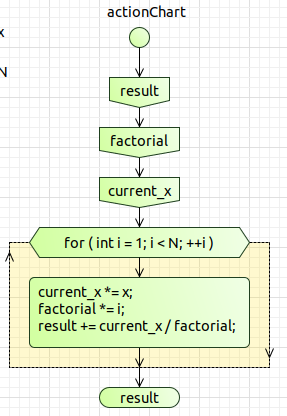
\includegraphics[scale=0.5]{exponent1}
	\caption{Диаграмма действий для суммы ряда экспоненты}
	\label{fig:exponent1}
\end{figure}

На вход данному алгоритму поступает количество итераций и степень $x$. (Рисунок \ref{fig:exponent2})
\begin{figure}[h]
	\centering 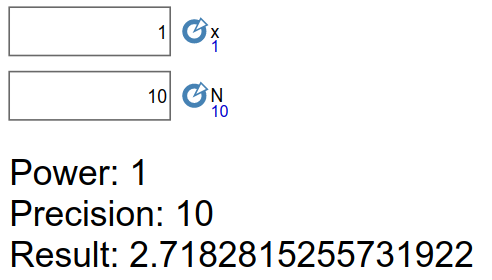
\includegraphics[scale=0.21]{exponent2}
	\caption{Результаты вычисления ряда экспоненты}
	\label{fig:exponent2}
\end{figure}

\newpage

Результаты расчёта совпали с результатами Wolfram Mathematica.\\

Таким образом, на примере создания функции для нахождения суммы ряда экспоненты был освоен процесс работы с диаграммами действий.